\documentclass[conference]{IEEEtran}
\IEEEoverridecommandlockouts
% The preceding line is only needed to identify funding in the first footnote. If that is unneeded, please comment it out.
\usepackage{cite}
\usepackage{amsmath,amssymb,amsfonts}
\usepackage{algorithmic}
\usepackage{graphicx}
\usepackage{textcomp}
\usepackage{xcolor}
\usepackage{tikz}
\usepackage{verbatim} 


\usetikzlibrary{positioning}
\def\BibTeX{{\rm B\kern-.05em{\sc i\kern-.025em b}\kern-.08em
    T\kern-.1667em\lower.7ex\hbox{E}\kern-.125emX}}
\begin{document}

\title{Machine Learning Autoencoder Applied to Communication Channels}


\author{\IEEEauthorblockN{Eduardo Dadalto Camara Gomes\IEEEauthorrefmark{1}}
\IEEEauthorblockA{\IEEEauthorrefmark{1}Institut Supérieur de l'Aéronautique et de l'Espace (ISAE-SUPAERO), Université de Toulouse, 31055 Toulouse, FRANCE\\
Email: eduardo.dadalto-camara-gomes@student.isae-supaero.fr}
}



\maketitle

\begin{abstract}

Communication channel error correction is key to enable digital critical communication systems to work efficiently. Although the optimal decoder for noisy channels, the maximum a posteriori (MAP) decoder, has already a mathematically proven optimal error probability minimization; its implementation cripples system applicability, since it introduces a large delay for large codewords. In this context, a deep neural network (DNN) is proposed to optimize the channel with an end-to-end autoencoder. The DNN autoencoder outperforms a MAP decoder form a given encoder in terms of delay, because of the first`s \textit{one-shot} capability once trained.

\end{abstract}

\begin{IEEEkeywords}
communication system, machine learning,  autoencoder, channel decoding, maximum a posteriori (MAP) decoder 
\end{IEEEkeywords}

\section{Introduction}
\subsection{Motivation}
A point to point communication channel is a system in which  two terminals exchange information through a noisy channel as Fig. \ref{fig:cs} illustrates. As a result of channel imperfections, Shannon theorized in \cite{b1} the ultimate reliable data rate that can be transmitted through a communication system with an arbitrarily small probability error. 

\begin{figure}[!ht]
  \centering
    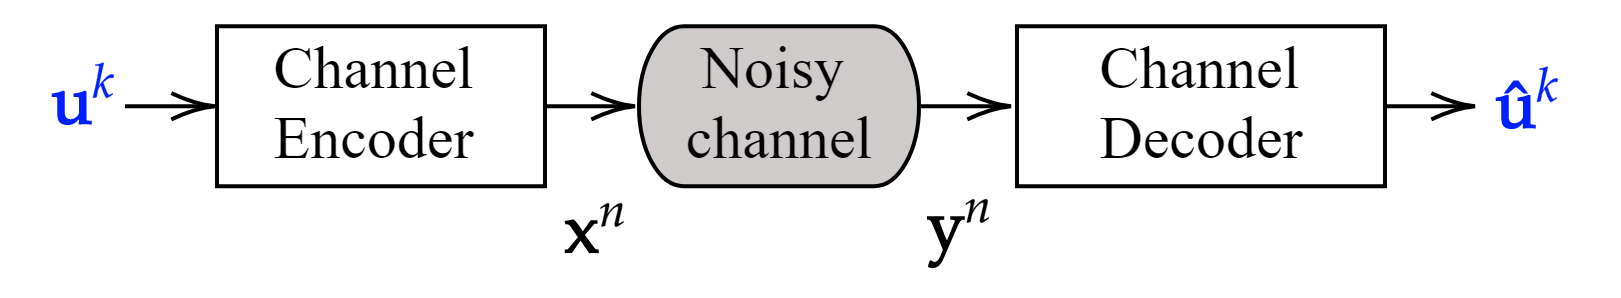
\includegraphics[width=0.5\textwidth]{simple_sys}
    \caption{Diagram of a simplified communication system.}\label{fig:cs}
\end{figure}

Since then, the research community in digital communication developed a series of algorithms to minimize error probability over a channel. In practice, the bit error rate (BER), an approximation of the probability of error, is targeted. However, the challenge of finding an \textit{efficient} solution  i.e., with both low latency and low error probability, for low signal to noise ratio (SNR) channels, remains. Low latency and high bandwidth wireless communication are key to critical systems, such as airplanes, satellites, cellular communication and 5G operations. The latter was studied by F. D. Calabrese et al. in \cite{b3} which  demonstrated that individual based radio resource management (RRM) algorithms were outperformed by a general learning framework, resulting in significant expense reductions, while increasing performance of the network.

Based on this vision, Tim O'Shea and Jakob Hoydis \cite{b2} pertinently noted that traditional algorithms in the field have foundations in probability theory e.g. maximum a posteriori (MAP) rule, maximum likelihood decoder (MLD) and turbo codes. Hence, they are usually built on top of mathematically convenient models. Even though they are theoretically optimal error corrector codes, these models often do not account for all the real system's imperfections, which leads to errors when implemented in practice.

As opposite to structured algorithms, machine learning (ML) algorithms do not require rigidly designed models and can take non-linearities effortlessly into account. These characteristics make these algorithms candidates for being used as channel decoder. Moreover, with ML based channel encoder and channel decoder, the design of communication systems as independently working blocks becomes obsolete, as a deep neural network (DNN) is able to actuate end-to-end in the system. As a result, an optimized autoencoder with a stochastic layer that models channel's imperfections can substitute the block based representation. Therefore, ML based communication systems could be a better representation of realistic systems and could optimize information transmission of different blocklengths and with low decoding latency, resulting ultimately in gain of bandwidth over standard methods. Thereby, ML algorithms are cardinal for state of the art communication applications. 

\subsection{Related work}

Recently, a significant amount of work in radio communication theory has emerged, introducing ML elements to the communication system. O'Shea et al. in \cite{osheaautoencoder} developed a channel autoencoder with optimized impairment and regularization layers to emulate channel impairments. They studied this architecture over an additive white Gaussian noise (AWGN) channel, founding ``some promising initial capacity" for this scheme. In their research, results in terms of BER over SNR for a DNN based autoencoder and for a convolutional neural network (CNN) based autoencoder were treated. They used a range of SNR - from $-10 \text{dB}$ to $15 \text{dB}$ - with QPSK and QAM16 modulation as benchmarks. This analysis was conducted for a binary input message.

    
T. Gruber et. al. in \cite{2018} proved that a deep learning-based channel decoder could actually learn a decoding algorithm rather than just being a simple classifier. They introduced codewords that were not been used in the training set, and the trained NN was able to correctly decode it. They also observed that structured codes are easier to learn than unstructured ones. NN for structured codes are able to generalize to the full codebook even if they have not seen all the training examples. They trained the NN for very short blocklengths ($N \leq 64$) in order to compare with MAP decoding performance.

\subsection{Problem statement}

In this work, we will implement a ML autoencoder for a  BSC that performs similar to the MAP decoder in real applications for a range of SNR from $-10 \text{dB}$ to $10 \text{dB}$. In its most simple form, a channel autoencoder includes an encoder, a noisy channel and a decoder. Using state-of-the art DNN algorithms to find the best solution of the problem, this work aims to contribute to set up a higher standard in terms of performance in bit-error correction and reduced delay for digital communication applications. In a near future, this disruptive methodology for error correction using ML could replace mathematically optimal decoders which are the current guideline.


%\subsection{Notation}
%Special notations used throughout the paper as shown in figures tac tac


\section{Theoretical Background}


\subsection{Maximum a posteriori decoder}


The concept of a MAP decoder algorithm for sequences, is choosing a message which maximizes the a posterior probability of the corrupted codeword $y$ received by the decoder \cite{b4}. This algorithm is known for its optimal error correction capability for white noise interference. This algorithm is also referred as the Viterbi decoder \cite{viterbi}.

Mathematically, we want to maximize the average probability of making a correct decision when analysing the channel output $\textbf{y}$, which is written as
\begin{equation}\label{eq:MAP1}
Pc := Pr[\textbf{X}=f({Y})]
\end{equation}
where $x \sim X$ and $y \sim Y$ are multivariate random variables. We derive below the decoder that maximizes $P_c$.

\begin{align} 
\Pr \left[ X=f\left( Y\right) \right]& =\sum_{f\left( y\right) y\in \mathcal{X}\times \mathcal{Y}} P_{XY}(f(y)y) \label{eq:MAP2} \\
&=\sum _{y\in \mathcal{Y}}P_{Y}\left( y\right)P_{X|Y}\left( f(y)|y\right) \label{eq:MAP3}
\end{align}

The optimal decoder is finally given by
\begin{align}
f(y) &= \underset{x\in \mathcal{X}}{\text{arg max}} P_{X|Y}(x|y)\label{eq:MAPF1}\\
&= \underset{x\in \mathcal{X}}{\text{arg max}}
P_X(x)P_{Y|X}(y|x).\label{eq:MAPF2}
\end{align}

However, the MAP decoder is practically nonviable to implement \cite{b6}. Thus, its variants cited in this paragraph are better suited for practical cases. The Log-MAP is an optimal decoder, having equivalent performance to the MAP decoder. While the Max-Log-MAP is a suboptimal decoder and will not be treated in this paper.  these variants are widely used as decoders for turbo codes \cite{b7}. Refer to \cite{b6} for specific details in the derivation of the Log-MAP algorithm. Furthermore, the Bahl-Cocke-Jelinek-Raviv (BCJR) algorithm is a bit-wise MAP rule with lower complexity widely used in practice, even for long data packets.

Turbo decoding using Log-MAP decoder for an additive white Gaussian noise (AWGN) channel and for a BSC was studied in \cite{b5}. They analyzed the BER for small SNR and concluded that the results are sensible to SNR estimation of the real channel, since the estimation of this parameter is required for the metric calculation of the algorithm \cite{b6}. It means that if the real SNR is smaller, the decoder will not perform well. Hence, for channel characteristics that change over time, the application of a MAP algorithm is debatable. This conclusion serve as motivation for ML autoencoders, which could adapt to different SNR conditions, outperforming the MAP decoder for realistic applications.

\subsection{Neural network basics}

\tikzset{%
  every neuron/.style={
    circle,
    draw,
    minimum size=0.666cm
  },
  neuron missing/.style={
    draw=none, 
    scale=2,
    text height=0.333cm,
    execute at begin node=\color{black}$\vdots$
  },
}

\begin{figure}[!hbp]
\centering

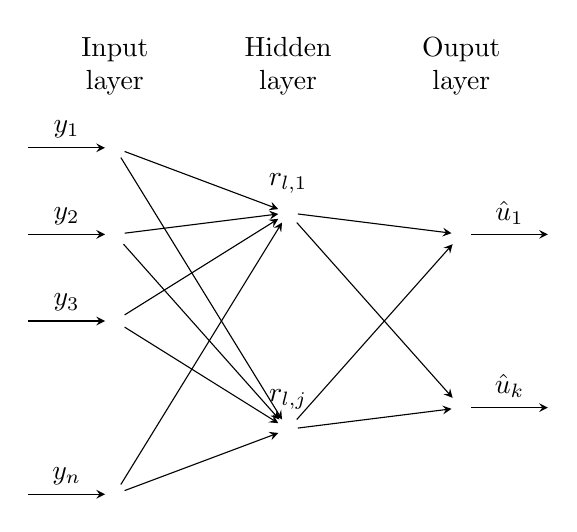
\begin{tikzpicture}[x=1.1cm, y=1.1cm, >=stealth]

\foreach \m/\l [count=\y] in {1,2,3,missing,4}
  \node [every neuron/.try, neuron \m/.try] (input-\m) at (0,2.5-\y) {};

\foreach \m [count=\y] in {1,missing,2}
  \node [every neuron/.try, neuron \m/.try ] (hidden-\m) at (2,2-\y*1.25) {};

\foreach \m [count=\y] in {1,missing,2}
  \node [every neuron/.try, neuron \m/.try ] (output-\m) at (4,1.5-\y) {};

\foreach \l [count=\i] in {1,2,3,n}
  \draw [<-] (input-\i) -- ++(-1,0)
    node [above, midway] {$y_\l$};

\foreach \l [count=\i] in {1,j}
  \node [above] at (hidden-\i.north) {$r_{l,\l}$};

\foreach \l [count=\i] in {1,k}
  \draw [->] (output-\i) -- ++(1,0)
    node [above, midway] {$\hat{u}_\l$};

\foreach \i in {1,...,4}
  \foreach \j in {1,...,2}
    \draw [->] (input-\i) -- (hidden-\j);

\foreach \i in {1,...,2}
  \foreach \j in {1,...,2}
    \draw [->] (hidden-\i) -- (output-\j);

\foreach \l [count=\x from 0] in {Input, Hidden, Ouput}
  \node [align=center, above] at (\x*2,2) {\l \\ layer};

\end{tikzpicture}

\caption{MLNN representative diagram, where $\textbf{y}^n$ is the input vector, $\textbf{r}_{l}^{j}$ is a hidden layer vector
and $\hat{\textbf{u}}^{k}$ is the output vector.} \label{fig:NN}
\end{figure}

Neural networks (NN) are a set of connected \textit{neurons} able to approximate any kind of function through an architecture composed of several single processing units (neurons) connected together forming a network. They are defined by \cite{b9} as parallel distributed, learning- and self-organizing information processing systems. 

In the context of learning algorithms implemented by a NN, the key issue is to find a suitable architecture that delivers the best results. To define and build this infrastructure, the activation function, the loss function and the structure must be decided. Nielson \cite{b8} in his book explores a vast amount of NN architectures and how they work. 

Multi-layer feed forward neural network (MLNN) as shown in Fig. \ref{fig:NN} will be applied in this work. They are known for the universal approximation property \cite{b9} and for the versatility of increasing the number of layers, creating a DNN able to undertake complex classification problems with low classification error and low dimensionality. In more general terms, a MLNN with $L$ layers, also called \textit{depth}, and parameter $\theta$ is a mapping of an input $\textbf{y}^n \in \mathbb{R}^{n}$ to an output $\textbf{û}^k \in \mathbb{R}^{k}$ through $L$ iterative steps. For a fully-connected network, each layer vector is calculated iteratively in the forward propagation. Each neuron is composed of a linear combiner and an activation function defined as 

\begin{equation}\label{eq:eqFP}
	f_{l}\left( \textbf{r}_{l-1};\theta _{l}\right) = \sigma \left( \textbf{W}_{l}\textbf{r}_{l-1}+\textbf{b}_{l}\right)
\end{equation}
where $\textbf{W}_{l}\in \mathbb{R} ^{N_{l}\times N_{l-1}}$ is the weight matrix between layers $l-1$ and $l$, $\textbf{r}_{l-1} \in \mathbb{R} ^{N_{l-1}}$ is a vector containing the hidden layer $l-1$ values, $\textbf{b}_{l}\in \mathbb{R} ^{N_l}$ is the bias vector and $\sigma$ is the activation function \cite{b2}.

% TODO: WRITE WHICH ACTIVATION FUNCTION I WILL USE
%

For a classification problem in communication, the \textit{categorical cross-entropy} loss function $l(\textbf{p},\textbf{q}):\mathbb{R} ^{N_L}\times \mathbb{R} ^{N_L}\mapsto \mathbb{R}$ defined in \eqref{eq:c-e} is most common. It is derived from the log-likelihood of a training set where $q_j$ is the estimated probability of the outcome $j$ and $p_{j}$ is the true probability. Basically, the function measures the dissimilarity between $p_{j}$ (what you expected) and $q_{j}$ (what you obtained) \cite{b10} where $j=1,...,N_L$.
\begin{equation}\label{eq:c-e}
	l(\textbf{p},\textbf{q})=-\sum _{j}p_{j}\log \left( q_{j}\right)
\end{equation}

With all these elements set, training the neural network to calculate an accurate weight matrix $\textbf{W}$ for forward propagation requires a labeled \textit{training data set}. This set is composed of pairs $ (\textbf{y}_{i}^{n}, {\mathbf{u}}_i^k) $, where $i=1,...,S$ and $S$ is the number of training sets. It matches the input and its respective desired output. The objective is to minimize the overall loss function defined in \eqref{eq:o-c-e} in terms of the parameter $\theta$ \cite{b2}. 
\begin{equation}\label{eq:o-c-e}
L\left( \theta \right) =\dfrac {1}{S}\sum ^{S}_{i=1}l\left({\mathbf{u}}_i^k  , \textbf{y}_{i}^{n}\right)	
\end{equation}  

This problem is an optimization problem and can be solved through different algorithms. For NN, an efficient way of computing this minimization is implementing the back-propagation (BP) algorithm. 	BP is classified as a supervised learning algorithm that is able to optimize a function based on some parameter and is highly parallelizable in computational terms \cite{b9}\cite{b8}.

One of the greatest advantage of NN is its ability to generalize the training set, delivering the right results even for input data not contained in the training set. With the weight matrix trained, the NN finds the correct output values for unseen inputs. In order to validate this principle, a \textit{validation data set} is used and the loss is mesured. Based on this value, we can evaluate the NN overall accuracy.

For implementing all the algorithms, Keras, a high-level python API for ML, will be used together with TensorFlow 1.13.1, a ML python friendly open-source library \cite{b11} \cite{b12}. Both are available on a free license terms.



\begin{comment}
\subsection{Autoencoders}
TO PARAPHRASE: The parallel computing
capabilities of NNs allow us to solve or, at least, approximate
the MLD problem in polynomial time [7]. Moreover, the
weights of the NN are precomputed during training and the
decoding step itself is then relatively simple. 

NNs which can learn an appropriate
mapping between noisy input patterns and codewords. No
assumption has to be made about the statistics of the channel
noise because the NN is able to learn the mapping or to
extract the channel statistics during the learning process

decoding problems have far more possibilities than conventional pattern recognition problems

In 2006, a new training technique, called layer-by-layer
unsupervised pre-training followed by gradient descent finetuning [14], led to the renaissance of NNs because it made
training of NNs with more layers feasible.

new hardware such as graphical processing units (GPUs) are available
to speed up learning as well as inference. In this renaissance
of NNs, new NND ideas emerge

The curse of dimensionality

\end{comment}
%\section{Procedure and methods}
%Explain what I Should do to achieve my goal
\begin{comment}

\subsection{Figures and Tables}


\begin{table}[htbp]
\caption{Table Type Styles}
\begin{center}
\begin{tabular}{|c|c|c|c|}
\hline
\textbf{Table}&\multicolumn{3}{|c|}{\textbf{Table Column Head}} \\
\cline{2-4} 
\textbf{Head} & \textbf{\textit{Table column subhead}}& \textbf{\textit{Subhead}}& \textbf{\textit{Subhead}} \\
\hline
copy& More table copy$^{\mathrm{a}}$& &  \\
\hline
\multicolumn{4}{l}{$^{\mathrm{a}}$Sample of a Table footnote.}
\end{tabular}
\label{tab1}
\end{center}
\end{table}


\begin{figure}[htbp]
\centerline{\includegraphics{fig1.png}}
\caption{Example of a figure caption.}
\label{fig}
\end{figure}
\end{comment}


\begin{thebibliography}{00}
\bibitem{b1} C. E. Shannon, ``A mathematical theory of communication," Bell System Technical Journal, vol. 27, no. 3, pp. 379–423, Jul. 1948.


\bibitem{b3} F. D. Calabrese, L. Wang, E. Ghadimi, G. Peters, and P. Soldati, ``Learning radio resource management in 5G networks: Framework, opportunities and challenges," arXiv preprint arXiv:1611.10253, 2016.

\bibitem{b2} O'Shea, Tim \& Hoydis, Jakob, ``An Introduction to Machine Learning Communications Systems", 2017.

\bibitem{osheaautoencoder} T. O'Shea, K. arra, T. C. Clancy, ``Learning to Communicate: Channel Auto-encoders, Domain Specific Regularizers, and Attention", 2016.

\bibitem{2018} T. Gruber, S. Cammerer, J. Hoydis, and S. ten Brink, “On deep learning based channel decoding,” accepted for CISS 2017, arXiv preprint arXiv:1701.07738, 2017.

\bibitem{b4} W. Alexander, H. Peter \& W. Norbert, ``Turbo-Decoding Without SNR Estimation",IEEE Communications Letter, vol. 4, no. 6, pp. 193-195, 2000.

\bibitem{viterbi} A. J. Viterbi, ``Error Bounds for Convolutional Codes and an Asymptotically Optimum Decoding Algorithm", IEEE Transactions on Information Theory, 13 (2): 260–269, 1967.

\bibitem{b6} Robertson, P. , Hoeher, P. and Villebrun, E. (1997), Optimal and sub‐optimal maximum a posteriori algorithms suitable for turbo decoding. Eur. Trans. Telecomm., 8: 119-125. doi:10.1002/ett.4460080202.

\bibitem{b7} J. Hagenauer,P. Robertson, L. Papke: iterative (“Turbo”) decoding of systematic convolutional codes with the MAP and SOVA
algorithms. In: ITG-Fachbericht 130. October 1994, p. 21-29.

\bibitem{b5} M. Jordan and R. Nichols, “The effects of channel characteristics on turbo code performance,” in Proc. Milcom’96, McLean, VA, Oct. 1996, pp. 17–21.

\bibitem{b9} I. Mohamed, ``Applications of neural networks to digital communications - a survey", 1997.

\bibitem{b8} M. Nielsen, \textit{Neural Networks and Deep Learning}.

\bibitem{b10} M. Kevin, ``Machine Learning: A Probabilistic Perspective", MIT, ISBN 978-0262018029, 2012.

\bibitem{b11} M. Abadi, A. Agarwal, P. Barham, et al., 
``TensorFlow: Large-scale machine learning on heterogeneous systems", 2015. Software available from tensorflow.org.

\bibitem{b12} F. Chollet, “keras,” https://github.com/fchollet/keras, 2015.



\end{thebibliography}



\end{document}
